\documentclass{article}
\usepackage{../settings}

\begin{document}
\hexcover{兩天一夜中南部行}{暑假作業}{作者:曾嘉禾}{Violet}{國文}

\begin{large}
\begin{boxpar}{第一站:彰化王功食海鮮}{Violet}
在從新竹出發後的剛開始,經過了彰化的王功。據說在那裡有神秘的宮廟文化,以及因為靠近海邊的關係而盛產海鮮。其中,店外大大的橫幅「蚵仔披薩」吸引了我的目光。所以我們一家人就去那家餐廳消費。雖然最後沒有點蚵仔披薩,但是店內的其他項目也十分誘人。例如鮮甜的絲瓜香菇,香氣十足的蛤蜊清湯,又大又肥的鮮蝦等。每一道菜經過味蕾後
\end{boxpar}
    \begin{boxpar}{第二站:嘉義}
    \end{boxpar}
    \begin{boxpar}{第三戰:台中雪山}
    \end{boxpar}

\begin{imgbox}{吃飯.jpg}
    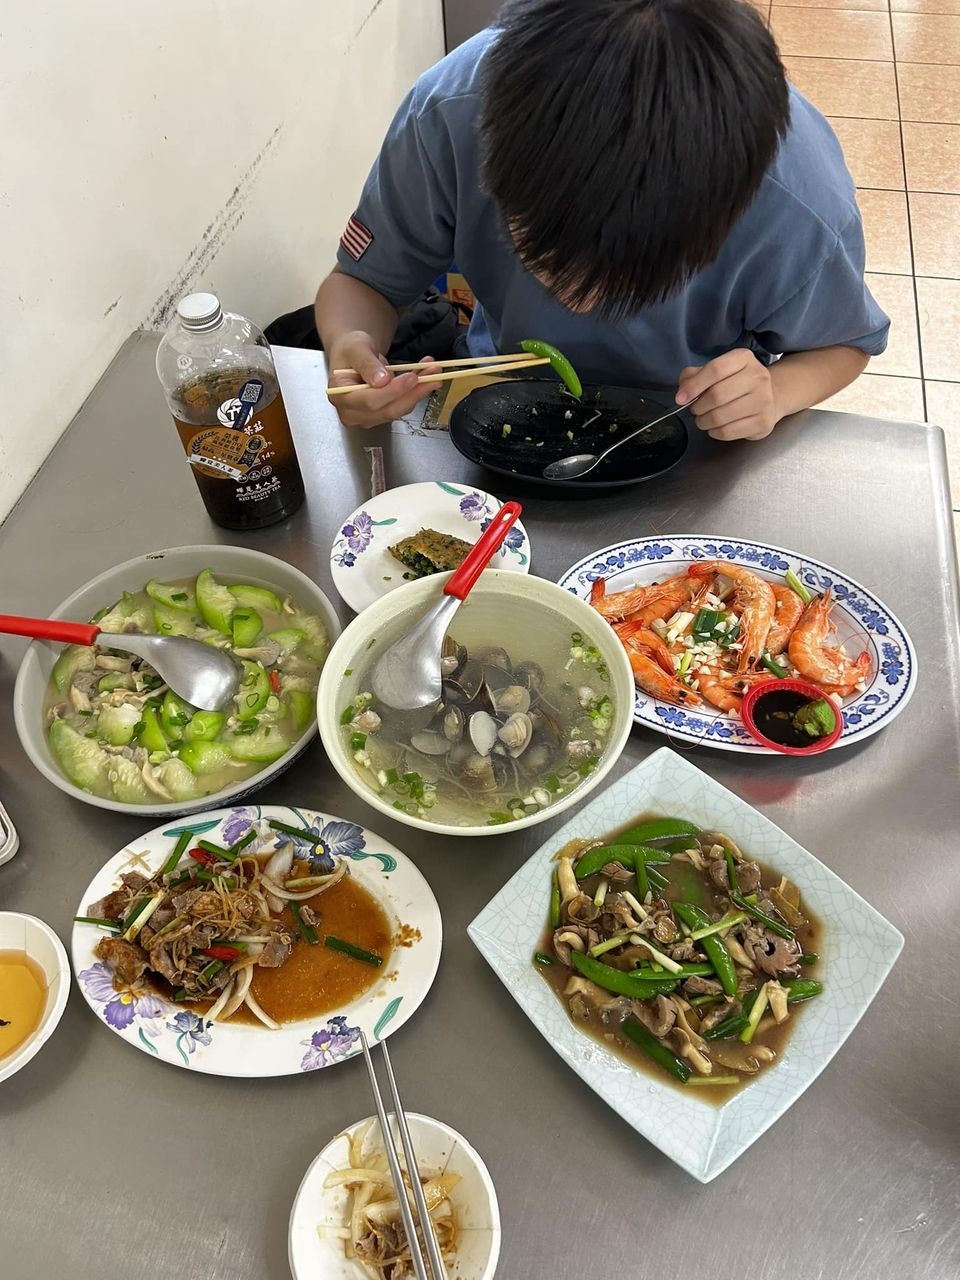
\includegraphics[width=0.65\textheight]{src/seafood.jpg}
\end{imgbox}
\end{large}
\end{document}
